\documentclass[10pt]{beamer}
\usefonttheme[onlymath]{serif}

\frenchspacing
\hyphenpenalty= 10000
\exhyphenpenalty= 10000

\usetheme[progressbar=frametitle]{m}

\usepackage{xcolor}
\definecolor{posterior}{RGB}{80, 110, 0}
\definecolor{prior}{RGB}{200, 0, 51}
\definecolor{likelihood}{RGB}{0, 140, 180}

\title{Markov Random Fields and Image Restoration}
%\subtitle{Gibbs Sampling and Annealing}
\date{\today}
\author{Alec Bunnell, Anne Grosse, Jialun Luo, Sam Spaeth}
\institute{Carleton College\\ Northfield, MN}

\begin{document}

\begin{frame}
\titlepage
\end{frame}

%%%%%%%%%%%%%%%%%%%%%%%%%%%%%%%%%%%%%%%%%%%%%%%%%%%%%%%%%%%%%%%%%%%%%%%%%%%%%%%%%%%%%
\section{Introduction}

%%%%%%%%%%%%%%%%%%%%%%%%%%%%%%%%%%%%%%%%%%%%%%%%%%%%%%%%%%%%%%%%%%%%%%%%%%%%%%%%%%%%%
\begin{frame}{Motivation}
Goal: Recover an image in its original quality, given only a noisy version of it.
\pause
\begin{center}
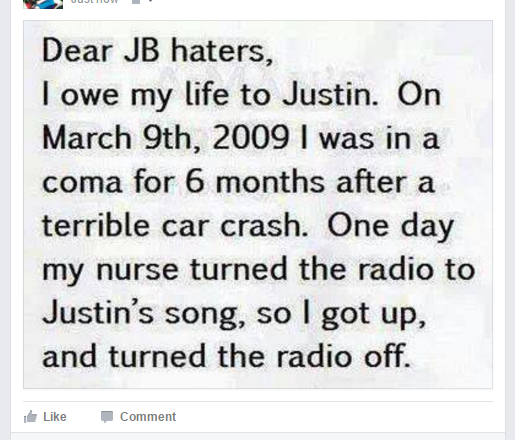
\includegraphics[scale=0.4]{img/bieber}
\end{center}
\end{frame}

%%%%%%%%%%%%%%%%%%%%%%%%%%%%%%%%%%%%%%%%%%%%%%%%%%%%%%%%%%%%%%%%%%%%%%%%%%%%%%%%%%%%%
\begin{frame}{Different Noise Models}
\begin{center}
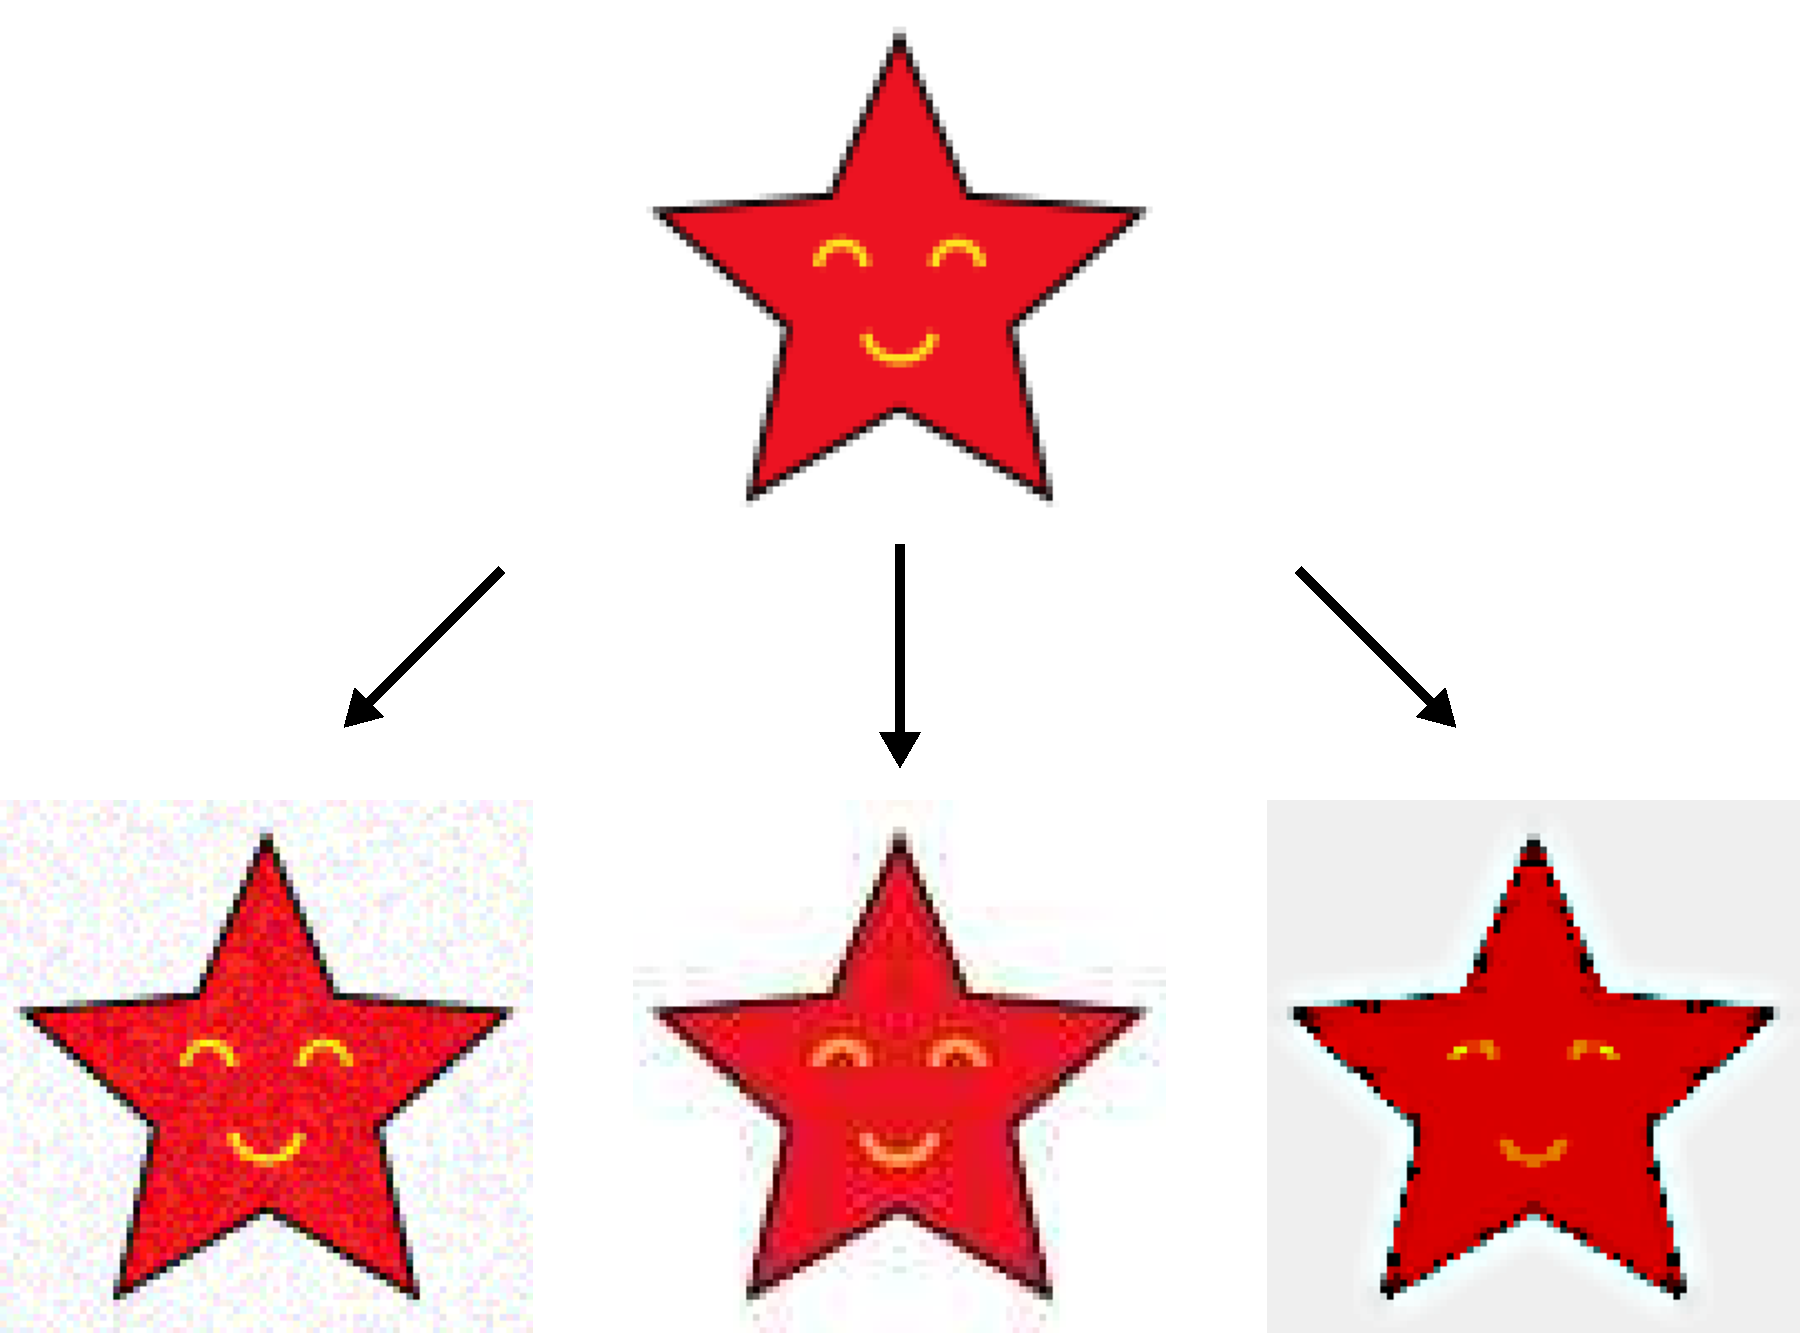
\includegraphics[scale=0.3]{img/allstars}
\end{center}
\end{frame}

%%%%%%%%%%%%%%%%%%%%%%%%%%%%%%%%%%%%%%%%%%%%%%%%%%%%%%%%%%%%%%%%%%%%%%%%%%%%%%%%%%%%% 
\begin{frame}{One Noise Model To Rule Them All}
\begin{block}{JPEG:}
\begin{itemize}
\item Uses lossy compression to reduce filesize, variable quality level
\item Designed to be relatively unnoticeable on photos (i.e., of real-life subjects)
\end{itemize}
\begin{center}
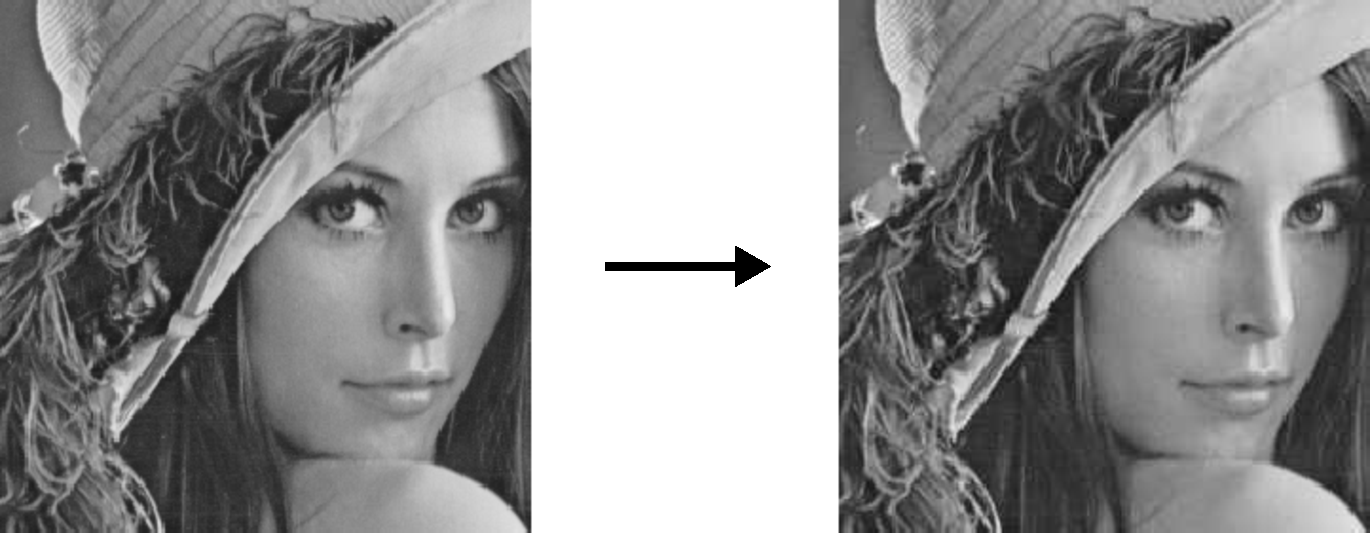
\includegraphics[scale=0.4]{img/yields-lena}
\end{center}
\end{block}
\end{frame}

\begin{frame}{One Noise Model To Rule Them All}
JPEG compression is significantly more noticeable on cartoon-like images and text.
\begin{center}

\includegraphics[scale=0.4]{img/yields-jpeg}
\end{center}
\end{frame}

%%%%%%%%%%%%%%%%%%%%%%%%%%%%%%%%%%%%%%%%%%%%%%%%%%%%%%%%%%%%%%%%%%%%%%%%%%%%%%%%%%%%%
\begin{frame}{Overview}
\begin{block}{Goal: Undo the error introduced by JPEG compression}
\begin{itemize}
\item Non-invertible compression
\item Best guess for the original image
\item Iteratively propose candidates, gradually improving towards our final recovered image
\end{itemize}
\end{block}
\end{frame}

%%%%%%%%%%%%%%%%%%%%%%%%%%%%%%%%%%%%%%%%%%%%%%%%%%%%%%%%%%%%%%%%%%%%%%%%%%%%%%%%%%%%%
\begin{frame}{Terminology}
\begin{block}{Image:}
%An image $x$ is a 2-D lattice of pixels, each of which has value $x_s \in [0, 1]$.

%(where $s \in V$, the set of all pixels.)
An image $x$ is a 2-D grid of pixels, each of which has value $x_s \in [0, 1]$ for $s\in V$, where $V$ is the set of pixels.
\begin{center}
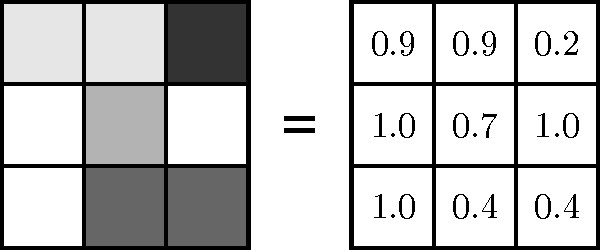
\includegraphics[scale=0.7]{img/lattice_def}
\end{center}
\end{block}

For now, we'll disregard color and work only in the grayscale setting.

\end{frame}

%%%%%%%%%%%%%%%%%%%%%%%%%%%%%%%%%%%%%%%%%%%%%%%%%%%%%%%%%%%%%%%%%%%%%%%%%%%%%%%%%%%%%
\begin{frame}{Terminology}
\begin{block}{Neighbors:}
We use the notation $t \sim s$ to say that $t$ is a neighboring pixel of $s$.

\begin{center}
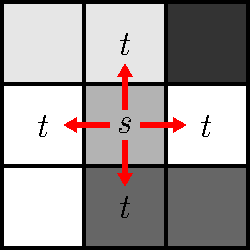
\includegraphics[scale=0.7]{img/lattice_neighbors}
\end{center}
\end{block}

For our purposes, we'll consider a pixel's neighbors to be the four pixels adjacent to it.
\end{frame}

%%%%%%%%%%%%%%%%%%%%%%%%%%%%%%%%%%%%%%%%%%%%%%%%%%%%%%%%%%%%%%%%%%%%%%%%%%%%%%%%%%%%%
\begin{frame}{Terminology}
\begin{block}{Notation:}
\begin{tabular}{l@{\hspace{0.1em}}l}
$y^*$ &$=$ the original, full quality image \\
$y$   &$=$ the given, degraded version of the original \\
$x$   &$=$ an arbitrary proposal image (a candidate for $x^*$) \\
$x^*$ &$=$ optimal candidate; our best attainable estimate of the original
\end{tabular}
\begin{center}
\begin{tabular}{cccc}

\includegraphics[scale=0.8]{results/bw-star} &

\includegraphics[scale=0.8]{results/bw-star-tmp2} &

\includegraphics[scale=0.8]{img/bw-star-sad} &

\includegraphics[scale=0.8]{results/bw-star}
\\ $y^*$ & $y$ & $x$ & $x^*$
\end{tabular}
\end{center}

Ideally, we would like our algorithm to produce $x^*\! = y^*\!$.
\end{block}
\end{frame}

%%%%%%%%%%%%%%%%%%%%%%%%%%%%%%%%%%%%%%%%%%%%%%%%%%%%%%%%%%%%%%%%%%%%%%%%%%%%%%%%%%%%%
\begin{frame}{A Small Simplification}
We'll start by considering a simpler noise model: i.i.d. additive Gaussian noise.
\begin{center}
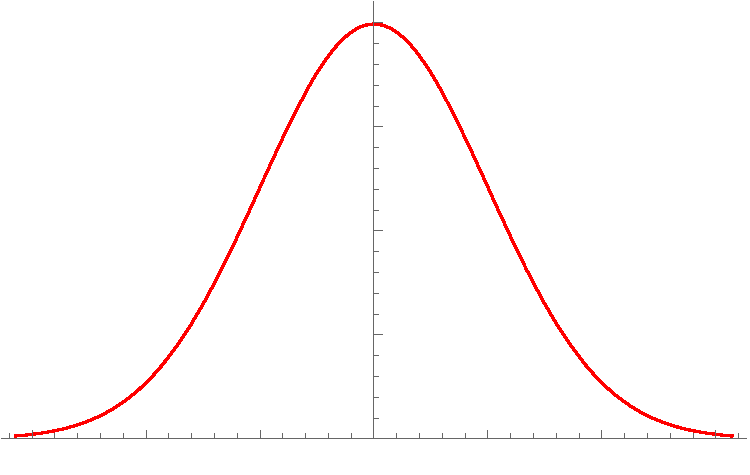
\includegraphics[scale=0.24]{img/normal}
\end{center}
Under this model, each pixel has an independent amount of normally-distributed jitter applied to it.
\begin{center}

\includegraphics[scale=0.3]{img/yields-gaussian}
\end{center}
\end{frame}



%%%%%%%%%%%%%%%%%%%%%%%%%%%%%%%%%%%%%%%%%%%%%%%%%%%%%%%%%%%%%%%%%%%%%%%%%%%%%%%%%%%%%
\section{The Energy Function}

%%%%%%%%%%%%%%%%%%%%%%%%%%%%%%%%%%%%%%%%%%%%%%%%%%%%%%%%%%%%%%%%%%%%%%%%%%%%%%%%%%%%%
\begin{frame}{A metric of image quality}
%We want to quantify the notion of what it means to be a ``good'' candidate.
%A metric on the space of images, $H(x)$, will determine the quality of an image $x$.

\begin{block}{Energy Function:}
$H(x)$ quantifies the ``quality'' of image $x$.
% : \text{space of images} \rightarrow \mathbb{R}$ such that
\end{block}

\begin{itemize}
\item $H(x)$ should be large (high energy) if $x$ is a bad candidate.
\item $H(x)$ should be small (low energy) if $x$ is more ideal.
\end{itemize}

\pause
\begin{center}
\begin{tabular}{ccc}

\includegraphics[scale=0.8]{results/bw-star} &

\includegraphics[scale=0.8]{results/bw-star-tmp} &

\includegraphics[scale=0.8]{img/bw-star-blobby}
\\ Original & Low Energy & High Energy
\end{tabular}
\end{center}
\end{frame}

%%%%%%%%%%%%%%%%%%%%%%%%%%%%%%%%%%%%%%%%%%%%%%%%%%%%%%%%%%%%%%%%%%%%%%%%%%%%%%%%%%%%%
\begin{frame}{Favoring smoothness}
What does a general image look like?
% A typical image has smooth transitions from pixel to pixel. To favor smoother candidates, we will penalize images with pixels that have values very different from their neighbors.
\begin{center}
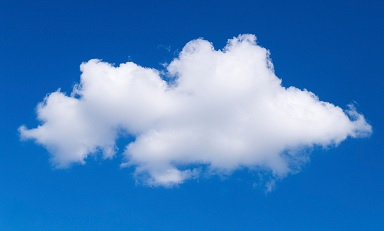
\includegraphics[scale=0.4]{img/cloud} \hspace{3em}
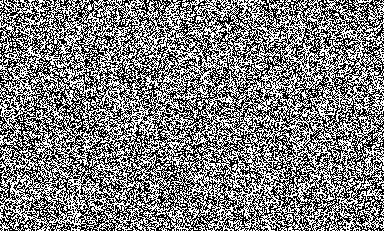
\includegraphics[scale=0.4]{img/static}
\end{center}

\end{frame}

%%%%%%%%%%%%%%%%%%%%%%%%%%%%%%%%%%%%%%%%%%%%%%%%%%%%%%%%%%%%%%%%%%%%%%%%%%%%%%%%%%%%%
\begin{frame}{Favoring smoothness}

We define $F$ to sum over a candidate image, comparing each pixel to its four neighboring pixels:
\[ F(x) = \sum_{s}f(s), \]
with 
\[f(s) = \sum_{t \sim s} (x_s - x_t)^2 \]

\pause
\begin{center}
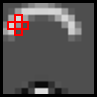
\includegraphics[scale=1.7]{img/compare_neighbors1}
\\ $x$
\end{center}
\end{frame}

%%%%%%%%%%%%%%%%%%%%%%%%%%%%%%%%%%%%%%%%%%%%%%%%%%%%%%%%%%%%%%%%%%%%%%%%%%%%%%%%%%%%%
\begin{frame}{Favoring smoothness}

We define $F$ to sum over a candidate image, comparing each pixel to its four neighboring pixels:
\[ F(x) = \sum_{s}f(s), \]
with 
\[f(s) = \sum_{t \sim s} (x_s - x_t)^2 \]

\begin{center}

\includegraphics[scale=1.7]{img/compare_neighbors2}
\\ $x$
\end{center}
\end{frame}

%%%%%%%%%%%%%%%%%%%%%%%%%%%%%%%%%%%%%%%%%%%%%%%%%%%%%%%%%%%%%%%%%%%%%%%%%%%%%%%%%%%%%
\begin{frame}{Perhaps a tad too smooth...}
If $H(x) = F(x)$, one minimizer of the function looks like:

\begin{center}

\includegraphics[scale=0.8]{results/bw-star-tmp}
\hspace{4em}

\includegraphics[scale=0.8]{img/bw-fail-nodata}
\end{center}

Any solid-color image would be an optimal (zero-energy) candidate for this choice of $H$.
\end{frame}

%%%%%%%%%%%%%%%%%%%%%%%%%%%%%%%%%%%%%%%%%%%%%%%%%%%%%%%%%%%%%%%%%%%%%%%%%%%%%%%%%%%%%
\begin{frame}{Incorporating the Given Data}
Solution: Penalize candidates that deviate far from the observed image. \pause Define:
\[ D(x) = \sum_{s}d(s), \]
with 
\[ d(s) = (x_s-y_s)^2 \]
\\[2ex]
\pause
\begin{center}
\begin{tabular}{c@{\hspace{3em}}c}
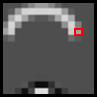
\includegraphics[scale=1.7]{img/compare_datax} &
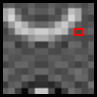
\includegraphics[scale=1.7]{img/compare_datay}
\\ $x$ & $y$
\end{tabular}
\end{center}
\end{frame}

%%%%%%%%%%%%%%%%%%%%%%%%%%%%%%%%%%%%%%%%%%%%%%%%%%%%%%%%%%%%%%%%%%%%%%%%%%%%%%%%%%%%%
\begin{frame}{Ignoring meaningful contrast}
Using $H(x) = F(x) + D(x)$ would produce something more like:

\begin{center}

\includegraphics[scale=0.8]{results/bw-star-tmp} 
\hspace{4em}

\includegraphics[scale=0.8]{img/bw-fail-robust}
\end{center}
(We can control the tradeoff between $F$ and $D$ by scaling $D(x)$ by some parameter $\theta$.)

We have balanced the over-smoothing with the noisy image, but there are still points in the image where no blurring should occur.

But not all contrast in an image is JPEG noise.

%When faced with contrast in the image, we would like to preserve ``meaningful'' contrast from the original image and smooth out artifacts that resulted from JPEG compression.

%We would like to smooth out JPEG noise but retain what we deem to be ``meaningful contrast''.

% Not all neighboring contrasts are products of noise process


%   "Previously, we posited that an ideal image exhibits smoothness: we would like each pixel to be similar to its neighbors.

%   Following this na\"ive prior, the optimal candidate would smooth out \textit{all} contrast in the noisy data, resulting in a blurry mess."

% Problem: Current energy function's ideal image would balance exhibiting smoothness and staying similar to the noisy data, resulting in a blurry mess. Sometimes there are abrupt intensity changes in an image.

\end{frame}

%%%%%%%%%%%%%%%%%%%%%%%%%%%%%%%%%%%%%%%%%%%%%%%%%%%%%%%%%%%%%%%%%%%%%%%%%%%%%%%%%%%%%
\begin{frame}{What is meaningful contrast?}

\begin{center}
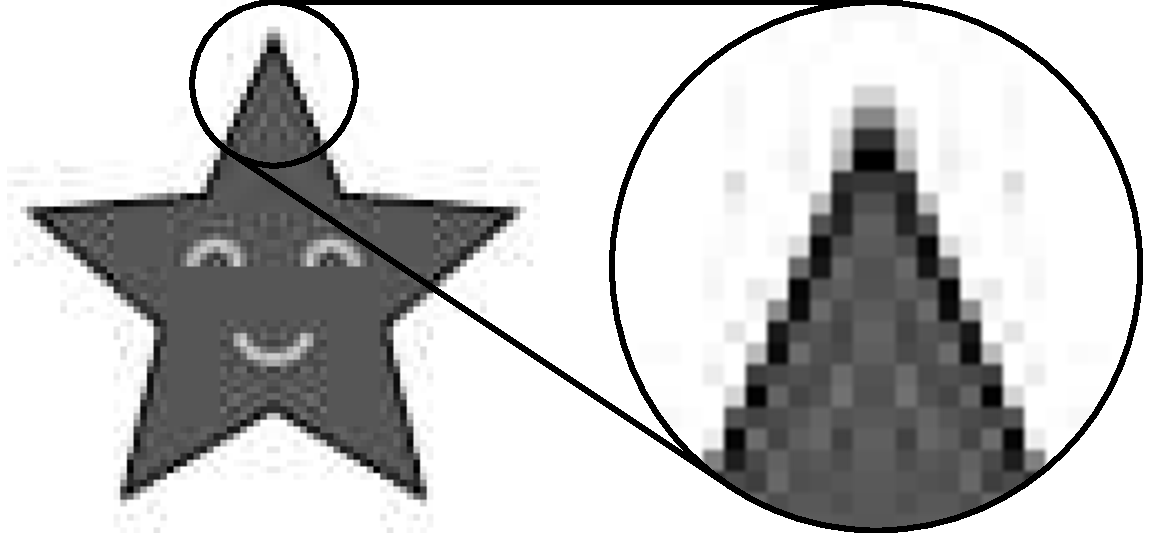
\includegraphics[scale=0.5]{img/noise_closeup}
\end{center}

\end{frame}

%%%%%%%%%%%%%%%%%%%%%%%%%%%%%%%%%%%%%%%%%%%%%%%%%%%%%%%%%%%%%%%%%%%%%%%%%%%%%%%%%%%%%
\begin{frame}{Preserving meaningful contrast}
Solution: Alter $F(x)=\sum\limits_{s}f(s)$ to tolerate great neighbor pixel differences.

% allow contrast if necessary.
\pause
\[ f(s) = \sum_{t \sim s} \left(|x_s-x_t|^{-2\alpha} + \gamma^{-\alpha}\right)^{-1/\alpha} \]

\begin{itemize}
\item $\gamma$ is the maximum penalty
\item $\alpha$ determines how quickly the penalty approaches the limit
\end{itemize}

\begin{center}
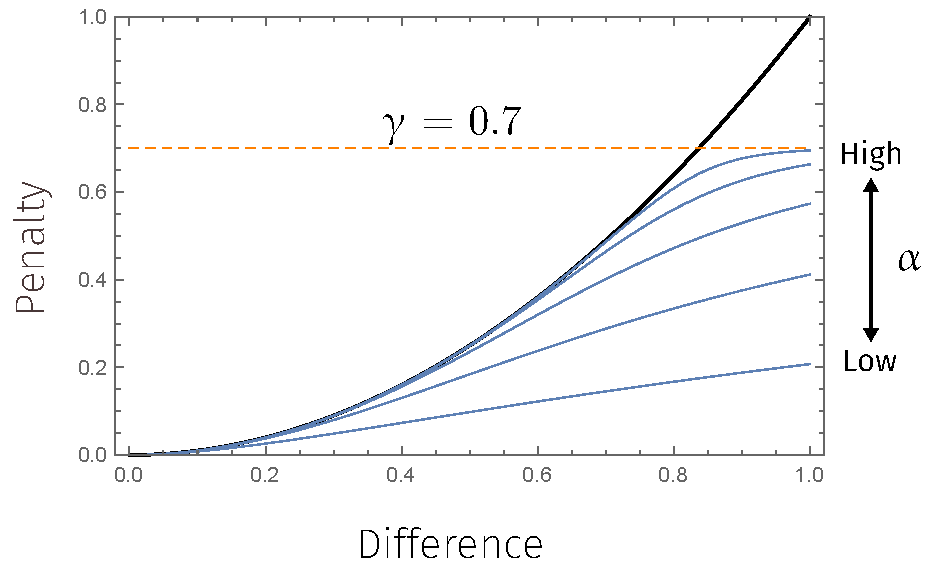
\includegraphics[width=0.6\linewidth]{img/alphagamma}
\end{center}

\end{frame}

%%%%%%%%%%%%%%%%%%%%%%%%%%%%%%%%%%%%%%%%%%%%%%%%%%%%%%%%%%%%%%%%%%%%%%%%%%%%%%%%%%%%%
\begin{frame}{Meaningful Contrast Preservation In Action}
The results are sensitive to our choice of $\gamma$ and $\alpha$:
\begin{center}
\begin{tabular}{c@{\hspace{1em}}c}

\includegraphics[width=9.5em]{img/fixed-hig-hia} &

\includegraphics[width=9.5em]{img/fixed-hig-loa} \\[0.5em]

\includegraphics[width=9.5em]{img/fixed-log-hia} &

\includegraphics[width=9.5em]{img/fixed-log-loa}
\end{tabular}
\end{center}

\end{frame}

%%%%%%%%%%%%%%%%%%%%%%%%%%%%%%%%%%%%%%%%%%%%%%%%%%%%%%%%%%%%%%%%%%%%%%%%%%%%%%%%%%%%%
\begin{frame}{Moving Forward}
Now that we have a satisfactory energy function, our goal is to minimize it.
\\[2ex]
Instead of directly searching for a minimizer, we'll use it to model the probability that a given candidate $x$ is the original image.
\end{frame}

%%%%%%%%%%%%%%%%%%%%%%%%%%%%%%%%%%%%%%%%%%%%%%%%%%%%%%%%%%%%%%%%%%%%%%%%%%%%%%%%%%%%%
\section{The Bayesian Paradigm}

%%%%%%%%%%%%%%%%%%%%%%%%%%%%%%%%%%%%%%%%%%%%%%%%%%%%%%%%%%%%%%%%%%%%%%%%%%%%%%%%%%%%%
\begin{frame}{Motivation}
\begin{itemize}
\item Consider an arbitrary candidate image $x$.
\item We would like to find $P(x \text{ original} \mid y \text{ observed})$ to assess how good of a guess $x$ is for the original image.
\pause
\item Using our noise model, $P(y \text{ observed} \mid x \text{ original})$ is straightforward.
\item Unfortunately, conditional probabilities aren't symmetric...
\end{itemize}
\end{frame}

%%%%%%%%%%%%%%%%%%%%%%%%%%%%%%%%%%%%%%%%%%%%%%%%%%%%%%%%%%%%%%%%%%%%%%%%%%%%%%%%%%%%%
\begin{frame}{Bayes' Rule}
Bayes' rule uses properties of conditional probability to provide a means for ``inverting'' a conditional probability $P(A \mid B) \rightarrow P(B \mid A)$.
\[ P(B \mid A) = \frac{P(A \cap B)}{P(A)} = \frac{P(A \mid B)P(B)}{P(A)} \]
\end{frame}

%%%%%%%%%%%%%%%%%%%%%%%%%%%%%%%%%%%%%%%%%%%%%%%%%%%%%%%%%%%%%%%%%%%%%%%%%%%%%%%%%%%%%
\begin{frame}{Bayes' Rule applied to images}
\begin{align*} P(x \text{ original} \mid y \text{ observed}) = \frac{P(y \text{ observed} \mid x \text{ original} ) P(x \text{ original})}{P(y \text{ observed})}
\end{align*}

Since $y$ is a fixed image (our observed data), we have
\textbf{
\[ \boldsymbol{ P(x \text{ original} \mid y \text{ observed}) \propto P(x \text{ original}) P(y \text{ observed} \mid x \text{ original}) } \] }

% \[ \underbrace{P(x \text{ original} \mid y \text{ observed})}_{{\color{posterior}\text{posterior}}} \propto \underbrace{P(x \text{ original})}_{{\color{prior}\text{prior}}} \underbrace{P(y \text{ observed} \mid x \text{ original})}_{{\color{likelihood}\text{likelihood}}} \]
\end{frame}

%%%%%%%%%%%%%%%%%%%%%%%%%%%%%%%%%%%%%%%%%%%%%%%%%%%%%%%%%%%%%%%%%%%%%%%%%%%%%%%%%%%%%
\begin{frame}{The Bayesian Paradigm}

\[ \underbrace{P(x \text{ original} \mid y \text{ observed})}_{{\color{posterior}\text{\normalsize{posterior}}}} \propto \underbrace{P(x \text{ original})}_{{\color{prior}\text{\normalsize{prior}}}} \underbrace{P(y \text{ observed} \mid x \text{ original})}_{{\color{likelihood}\text{\normalsize{likelihood}}}} \]

\begin{block}{Main Idea:}
\begin{itemize}
\item Begin with some {\color{prior}prior} expectations about what you think a general image should look like.
\item Take into account the {\color{likelihood}likelihood} of obtaining the given degraded image assuming that things started from our candidate.
\item Yield an updated, {\color{posterior}posterior} probability distribution describing our candidate.
\end{itemize}
\end{block}
\end{frame}

%%%%%%%%%%%%%%%%%%%%%%%%%%%%%%%%%%%%%%%%%%%%%%%%%%%%%%%%%%%%%%%%%%%%%%%%%%%%%%%%%%%%%
\begin{frame}{The Energy Function Strikes Back}
\begin{itemize}
\item Recall: We would like to find a candidate image $x$ such that it minimizes our energy function $H(x)$.
\item We'll construct a probability distribution in which low energy candidates are the most likely.
\item Use $\Pi(x) \propto e^{-H(x)}$.
\end{itemize}
\end{frame}

%%%%%%%%%%%%%%%%%%%%%%%%%%%%%%%%%%%%%%%%%%%%%%%%%%%%%%%%%%%%%%%%%%%%%%%%%%%%%%%%%%%%%
\begin{frame}{Back to the Bayes-ics}
\begin{align*}
{\color{posterior}\Pi(x)} &\propto e^{-H(x)}
\\ &\propto e^{-F(x) - D(x)}
\\ &\propto {\color{prior}e^{-F(x)}} {\color{likelihood}e^{-D(x)}}
\end{align*}

Observe that 
\begin{itemize}
\item {\color{prior}$F(x)$} describes the energy \textit{within} the candidate, based on our prior expectations of what makes an image ``ideal'' ({\color{prior}prior})
\item {\color{likelihood}$D(x)$} disallows the candidate from straying too far from the observed data ({\color{likelihood}likelihood})
\item {\color{posterior}$\Pi(x)$} will favor candidates that satisfy both of these conditions in an optimally balanced way ({\color{posterior}posterior})
\end{itemize}

\end{frame}

%%%%%%%%%%%%%%%%%%%%%%%%%%%%%%%%%%%%%%%%%%%%%%%%%%%%%%%%%%%%%%%%%%%%%%%%%%%%%%%%%%%%%
\begin{frame}{Our Posterior Distribution}
\begin{block}{}
We thus have the following model for the probability that a candidate $x$ is our source image, given only the degraded image $y$:
\pause
\begin{align*}
\Pi(x) &\propto e^{-H(x)}
\\ &\propto e^{-\sum\limits_{s} \left(\sum\limits_{t \sim s} \left(|x_s-x_t|^{-2\alpha} + \gamma^{-\alpha}\right)^{-1/\alpha} +\, \theta(x_s-y_s)^2\right)}
\end{align*}
\end{block}
\end{frame}

%%%%%%%%%%%%%%%%%%%%%%%%%%%%%%%%%%%%%%%%%%%%%%%%%%%%%%%%%%%%%%%%%%%%%%%%%%%%%%%%%%%%%
\begin{frame}{Sampling from the Posterior}
We have now constructed a distribution on the space of images such that ``better'' images are considered more likely.
\\[2ex]
If we could sample from $\Pi$, we'd get these ``better'' images most often.
\\[2ex]
Sampling images according to $\Pi$ would be a fine way of proposing candidates!

\end{frame}

%%%%%%%%%%%%%%%%%%%%%%%%%%%%%%%%%%%%%%%%%%%%%%%%%%%%%%%%%%%%%%%%%%%%%%%%%%%%%%%%%%%%%
\begin{frame}{``Houston, we have a problem''}
To sample from $\Pi$ directly, we must enumerate the space of all possible images and find the constant of proportionality.
\begin{itemize}
\pause \item For an $R \times C$ image stored with $k$ discrete gray levels, there are $k^{RC}$ unique image possibilities.
\pause \item At $256$ gray-levels (standard), even a $6\times 6$ image has $256^{6\times 6} \sim 10^{86}$ possibilities.
\pause \item As a comparison, the estimated number of particles in the known universe is $\sim 10^{80}$.
\end{itemize}
\pause 
So sampling from $\Pi$ will be a bit of a challenge...
\end{frame}

%%%%%%%%%%%%%%%%%%%%%%%%%%%%%%%%%%%%%%%%%%%%%%%%%%%%%%%%%%%%%%%%%%%%%%%%%%%%%%%%%%%%%
\section{The Gibbs Sampler}

%%%%%%%%%%%%%%%%%%%%%%%%%%%%%%%%%%%%%%%%%%%%%%%%%%%%%%%%%%%%%%%%%%%%%%%%%%%%%%%%%%%%%
\begin{frame}{The Gibbs Sampler}
\begin{itemize}
\item Treat each pixel's value $x_s$ as a random variable $X_s$.
\item A random image is a collection of these random pixels, $X = (X_s)_{s \in V}$.
\item The Gibbs Sampler allows sampling from a joint distribution of random variables. 
\item The distribution of a random image $X$ is simply the joint distribution of all its pixels.
\end{itemize}
\end{frame}

%%%%%%%%%%%%%%%%%%%%%%%%%%%%%%%%%%%%%%%%%%%%%%%%%%%%%%%%%%%%%%%%%%%%%%%%%%%%%%%%%%%%%
\begin{frame}{How it works}
Instead of proposing a completely new candidate at each iteration, propose a new image by changing one pixel at a time.

Steps:
\begin{itemize}
\item Randomly choose a pixel $s$ to update.
\item Find the distribution of $X_s \mid X_t, \forall t \neq s$.
\item Randomly select a new value for $x_s$ according to this distribution.
\item Repeat.
\end{itemize}
%This gives us the ability to sample from $\Pi$ if we can the abov 
\end{frame}

%%%%%%%%%%%%%%%%%%%%%%%%%%%%%%%%%%%%%%%%%%%%%%%%%%%%%%%%%%%%%%%%%%%%%%%%%%%%%%%%%%%%%
\begin{frame}{One more problem}
The conditional distribution of $X_s \mid X_t, \forall t \neq s$  is not immediately obvious...
\end{frame}

%%%%%%%%%%%%%%%%%%%%%%%%%%%%%%%%%%%%%%%%%%%%%%%%%%%%%%%%%%%%%%%%%%%%%%%%%%%%%%%%%%%%%
\section{Markov Random Fields}

%%%%%%%%%%%%%%%%%%%%%%%%%%%%%%%%%%%%%%%%%%%%%%%%%%%%%%%%%%%%%%%%%%%%%%%%%%%%%%%%%%%%%
\begin{frame}{The Markov Chain}
\begin{block}{Definition}
A Markov Chain is a sequence of random variables $X_1, X_2, \ldots$ that satisfies
\[ P(X_{n+1} = x_{n+1} \mid X_1 = x_1, \ldots, X_n = x_n) \,=\, P(X_{n+1} = x_{n+1} \mid X_n = x_n) \]
for all steps $n$. 
\pause
\textbf{At each point in the chain, the next step is dependent only on the current step, regardless of all other steps.}
\\[2ex]
 \pause This is known as the \textbf{Markov property} for Markov chains. 
\end{block}
\pause
\begin{figure}
\centering
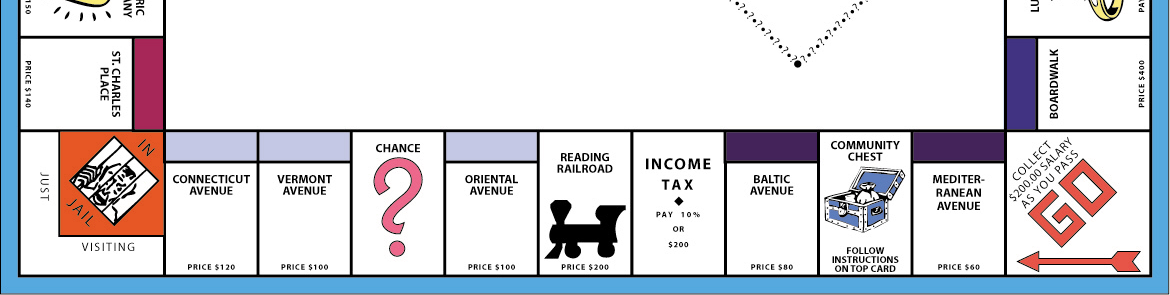
\includegraphics[width = 0.6\linewidth]{img/monopoly.png}
\end{figure}
\end{frame}

%%%%%%%%%%%%%%%%%%%%%%%%%%%%%%%%%%%%%%%%%%%%%%%%%%%%%%%%%%%%%%%%%%%%%%%%%%%%%%%%%%%%%
\begin{frame}{Image as a Graph}
%We'll generalize our treatment of an image to that of a graph with vertices $V$ and edges connecting them.

An image can be represented by a graph with vertices $V$ and edges connecting adjacent pixels.

\begin{center}
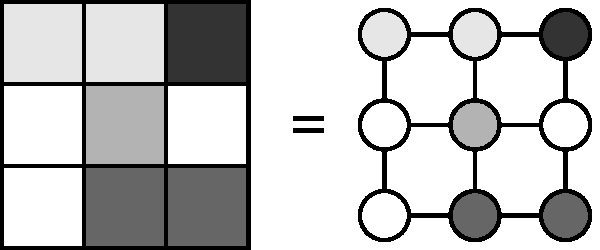
\includegraphics[scale=0.7]{img/lattice_graph}
\end{center}

Recall that the value of pixel $s$ (now vertex $s$) is a random variable $X_s$.

%This yields random variable $X_s$.
% Let $\mathbb{X}$ be the space of all possible configurations.
\end{frame}

%%%%%%%%%%%%%%%%%%%%%%%%%%%%%%%%%%%%%%%%%%%%%%%%%%%%%%%%%%%%%%%%%%%%%%%%%%%%%%%%%%%%%
\begin{frame}{The Markov Random Field}
A Markov Random Field is a graph that satisfies
\[ P(X_s = x_s \mid X_t = x_t, \forall t \neq s) \,=\, P(X_s = x_s \mid X_t = x_t, \forall t \sim s) \]
for all configurations $X$.
\\[2ex]
This is analogous to the Markov Property defined for Markov Chains.
\\[2ex]
\textbf{The probability distribution for one vertex given the entire configuration requires us to look no further than its neighbors.}
\end{frame}

%%%%%%%%%%%%%%%%%%%%%%%%%%%%%%%%%%%%%%%%%%%%%%%%%%%%%%%%%%%%%%%%%%%%%%%%%%%%%%%%%%%%%
\begin{frame}{Hammersley--Clifford Theorem}
\begin{block}{Theorem (Hammersley--Clifford):}
A probability distribution with respect to a graph structure imposes a Markov Random Field if and only if the distribution is Gibbsian.
\end{block}

\begin{center}
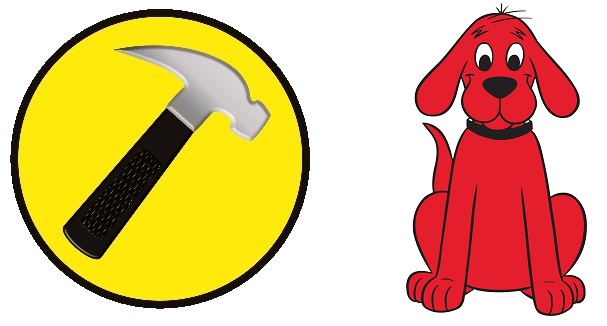
\includegraphics[width = 0.5\linewidth]{img/hammersley-clifford}
\end{center}
 \end{frame}

%%%%%%%%%%%%%%%%%%%%%%%%%%%%%%%%%%%%%%%%%%%%%%%%%%%%%%%%%%%%%%%%%%%%%%%%%%%%%%%%%%%%%
\begin{frame}{Gibbsian Distribution}
\begin{block}{Definition:}
A distribution $\Pi$ is \textbf{Gibbsian} if and only if $\Pi(x) \propto e^{-H(x)}$, where:
\begin{itemize}
\item $H(x)$ is a strictly positive function \\[1.5ex]
%measure on a configuration $x$
\item $H(x) = \sum\limits_s h(s)$, where $h(s)$ depends only on $t\sim s$.
%\item The calculation of $h(s)$ only depends on the vertices $t \sim s$.
\end{itemize}
\end{block}

\pause
Our posterior distribution: 
\[ \Pi(x) \propto e^{-H(x)} = e^{-\sum\limits_s h(s)} \]
where $h(s) = f(s) + d(s)$.\\[2ex]
\textbf{Thus, our energy function imposes a Markov Random Field on an arbitrary image}% over the space of all image configurations.}


\end{frame}

%%%%%%%%%%%%%%%%%%%%%%%%%%%%%%%%%%%%%%%%%%%%%%%%%%%%%%%%%%%%%%%%%%%%%%%%%%%%%%%%%%%%%
\begin{frame}{The Mysterious Conditional Revisited}
Since we have a Markov Random Field, the Markov Property must hold for our choice of $\Pi$.
Specifically, we have that
\begin{align*}
P(X_s = x_s \mid X_t = x_t, \forall t \neq s) \,&=\, P(X_s = x_s \mid X_t = x_t, \forall t \sim s) 
\\ &\propto e^{-h(s)}
\end{align*}
% \alert{talk about proportionality}
% \\[2ex]
Thus, to implement the Gibbs sampler, only calculations using the neighbors of a pixel $s$ are required to update that pixel.
\end{frame}

%%%%%%%%%%%%%%%%%%%%%%%%%%%%%%%%%%%%%%%%%%%%%%%%%%%%%%%%%%%%%%%%%%%%%%%%%%%%%%%%%%%%%
\begin{frame}{Sampling vs Recovering}
\begin{itemize}
\item Due to the Gibbs sampler, we can now \textit{sample} images from $\Pi$.
\item However, we don't just want a sample of images which are just ``likely'' to have low energy; we want to produce \textit{one} image that has the \textit{lowest} energy.
\item This is called the \textit{maximum a posteriori} (MAP) estimate.
\end{itemize}
\end{frame}

%%%%%%%%%%%%%%%%%%%%%%%%%%%%%%%%%%%%%%%%%%%%%%%%%%%%%%%%%%%%%%%%%%%%%%%%%%%%%%%%%%%%%
\section{Simulated Annealing}
%%%%%%%%%%%%%%%%%%%%%%%%%%%%%%%%%%%%%%%%%%%%%%%%%%%%%%%%%%%%%%%%%%%%%%%%%%%%%%%%%%%%%
\begin{frame}{Annealing}
%Simulated annealing is inspired by the technique of annealing in metalsmithing, where the metal being worked on is gradually cooled.

\begin{center} 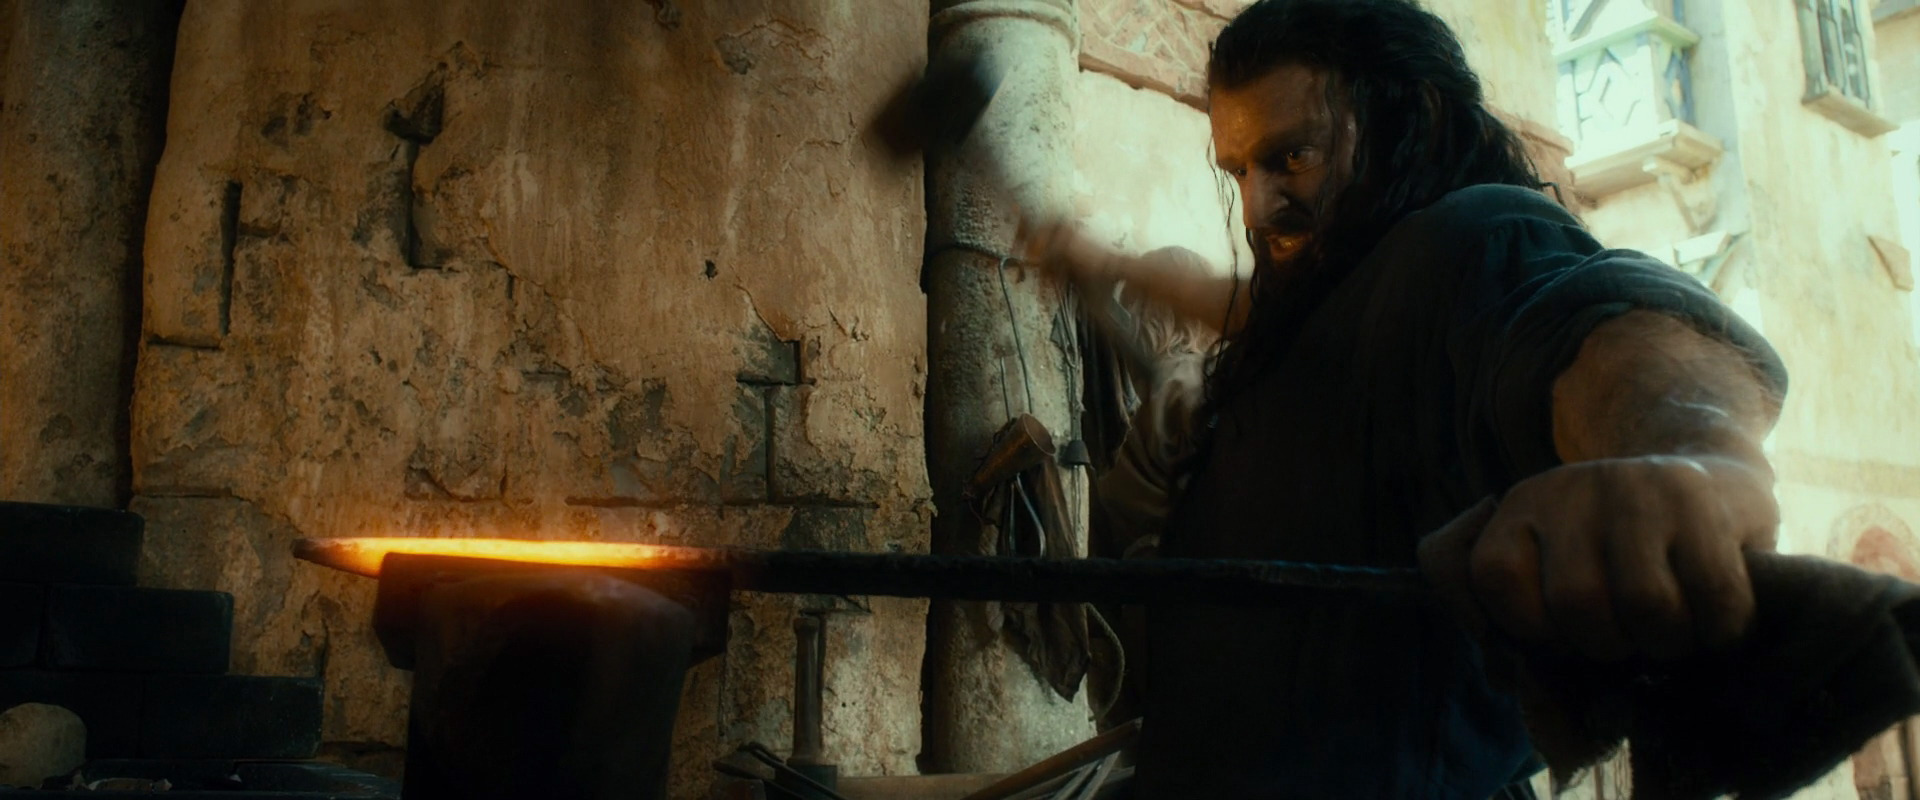
\includegraphics[width = 0.9\linewidth]{img/thorin-blacksmith.jpg} \end{center}

%Annealing is used to allow metals to achieve an equilibrium state.
\end{frame}

%%%%%%%%%%%%%%%%%%%%%%%%%%%%%%%%%%%%%%%%%%%%%%%%%%%%%%%%%%%%%%%%%%%%%%%%%%%%%%%%%%%%%
\begin{frame}{Simulated Annealing}
\vspace{1ex}
Introduce parameter $\beta$ to our posterior distribution: $e^{-\beta H(x)}$.

By varying $\beta$, we can control how ``peaked'' our distribution is.
\\[4ex]

\pause

\begin{center}
\begin{tabular}{ccc}
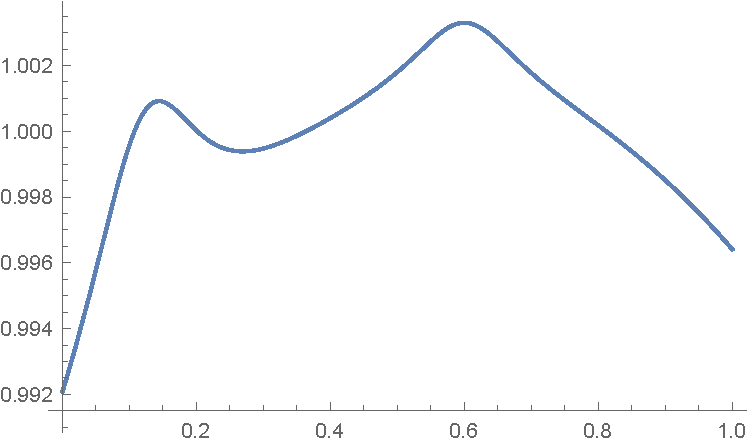
\includegraphics[width=0.3\linewidth]{img/anneal-beta1} &
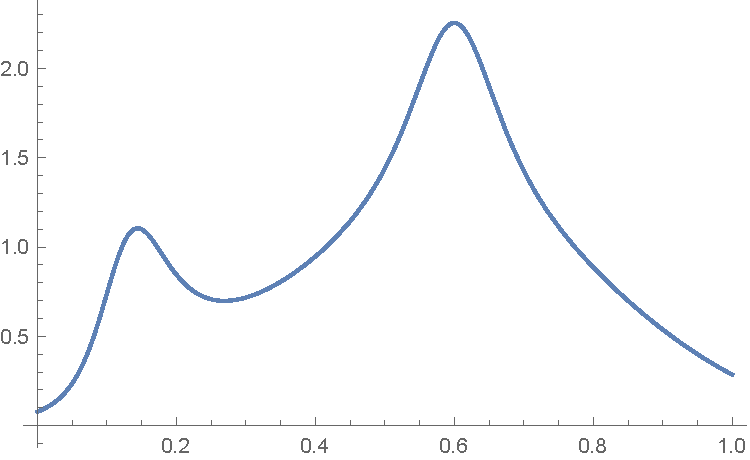
\includegraphics[width=0.3\linewidth]{img/anneal-beta300} &
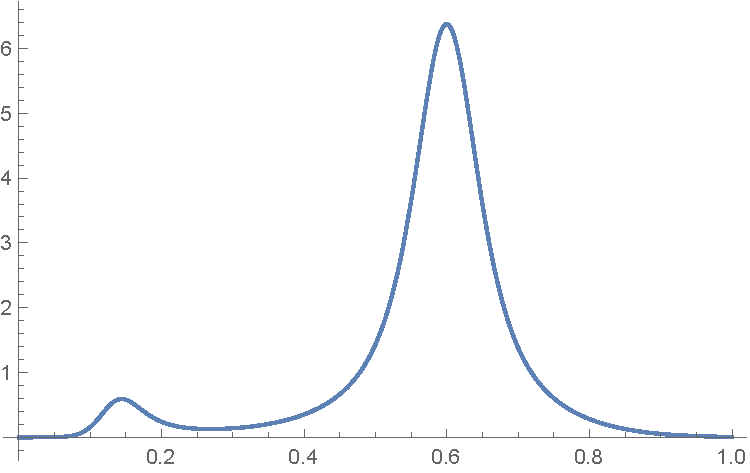
\includegraphics[width=0.3\linewidth]{img/anneal-beta1000} \\
$\beta = 1$ & $\beta = 300$ & $\beta = 1000$
\end{tabular}
\end{center}

\pause

We'll call this parameter inverse temperature.
\begin{itemize}
\item High ``temperature'' (low $\beta$) = lots of ``jumping around''
\item Low ``temperature'' (high $\beta$) = not as much ``movement''
\end{itemize}
\end{frame}

%%%%%%%%%%%%%%%%%%%%%%%%%%%%%%%%%%%%%%%%%%%%%%%%%%%%%%%%%%%%%%%%%%%%%%%%%%%%%%%%%%%%%
\begin{frame}{The Cooling Schedule}
%In the real world, reducing the temperature of the metal too quickly would cause cracking and ruin the metal.
%\\[2ex]
%Similarly, ``cooling down'' too quickly in the Gibbs sampler can lock you into a local minimum.
%\\[2ex]

\begin{block}{Cooling Schedule}
A sequence of inverse temperatures $\beta_1,\ldots,\beta_n,\ldots$ modifying the posterior distribution $\Pi$ is called a cooling schedule.

So at $n$th step, the posterior distribution is given by $\Pi(x) \propto e^{-\beta_n H(x)}$.

Our Gibbs Sampler conditional likewise becomes proportional to $e^{-\beta_n h(s)}$.
\end{block}


%A cooling schedule defines the inverse temperature $\beta_n$ used at the $n$th step of the chain.
%\\[2ex]
%Remarkably, it's possible to derive a cooling schedule that guarantees that we'll lock into the \textit{global} minimum energy image.
% Analogy to metal-smithing: 


\end{frame}

%%%%%%%%%%%%%%%%%%%%%%%%%%%%%%%%%%%%%%%%%%%%%%%%%%%%%%%%%%%%%%%%%%%%%%%%%%%%%%%%%%%%%
\begin{frame}{Finding the global minimum}
\begin{block}{Theorem (Geman \& Geman)}
If a cooling schedule $\beta_1,\ldots,\beta_n,\ldots$ satisfies
\[ \beta_n \leq \frac{1}{RC(\gamma+\theta)}\log n \]
then we will eventually sample the mode of the posterior distribution (or the minimum-energy image) with probability 1.
\end{block}
\end{frame}

%%%%%%%%%%%%%%%%%%%%%%%%%%%%%%%%%%%%%%%%%%%%%%%%%%%%%%%%%%%%%%%%%%%%%%%%%%%%%%%%%%%%%
\section{Implementation and Adaptations}

%%%%%%%%%%%%%%%%%%%%%%%%%%%%%%%%%%%%%%%%%%%%%%%%%%%%%%%%%%%%%%%%%%%%%%%%%%%%%%%%%%%%%
\begin{frame}{Modified Cooling Schedule}
%Unfortunately, this cooling schedule is unbearably slow and infeasible in practice, but using a faster cooling schedule still gives reasonable empirical results.
\pause \begin{center}
\begin{tabular}{ccc}
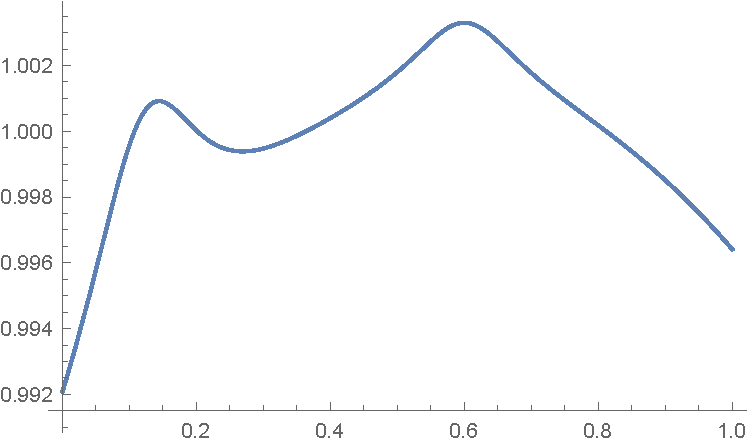
\includegraphics[width=0.3\linewidth]{img/anneal-beta1} &
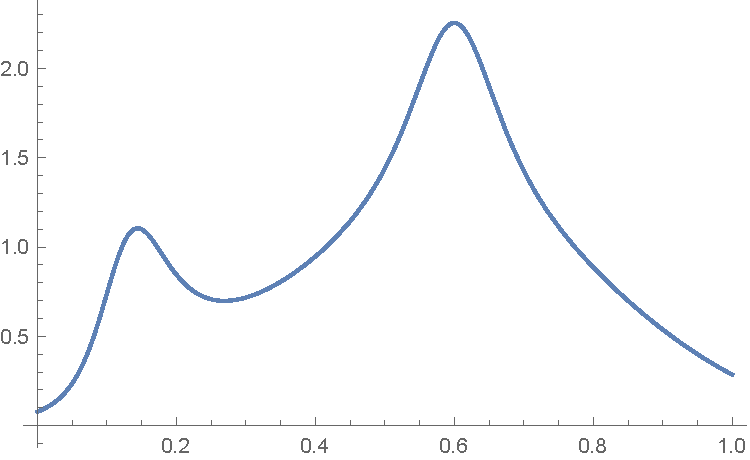
\includegraphics[width=0.3\linewidth]{img/anneal-beta300} &
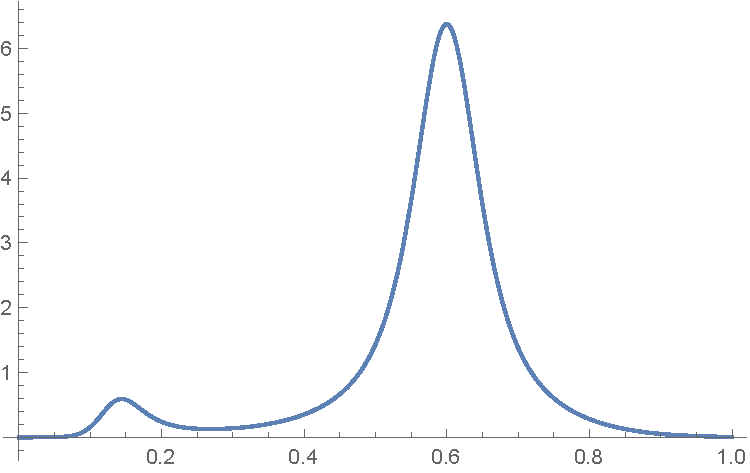
\includegraphics[width=0.3\linewidth]{img/anneal-beta1000} \\
$\beta = 1$ & $\beta = 300$ & $\beta = 1000$
\end{tabular}
\end{center}
\begin{itemize}
\pause \item Sticking to the exact bound given by Geman--Geman is incredibly slow. 
\pause \item Geman--Geman's theorem assumes that the starting candidate is random noise.
\end{itemize}
\pause
We introduce parameter $\tau$ to control our cooling schedule:
\[ \beta_n = \tau \log n \]

\end{frame}

%%%%%%%%%%%%%%%%%%%%%%%%%%%%%%%%%%%%%%%%%%%%%%%%%%%%%%%%%%%%%%%%%%%%%%%%%%%%%%%%%%%%%
\begin{frame}{Gibbs Sampler Results}
\centering
\begin{tabular}{c@{\hspace{.5em}}c@{\hspace{.5em}}c}
Original image & Noisy Data & MAP estimate \\[2ex]

\includegraphics[width=9.5em]{results/bw-star} 
&
\includegraphics[width=9.5em]{results/bw-star-tmp}
&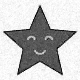
\includegraphics[width=9.5em]{results/bw-star-gibbs}
\end{tabular}
\end{frame}

%%%%%%%%%%%%%%%%%%%%%%%%%%%%%%%%%%%%%%%%%%%%%%%%%%%%%%%%%%%%%%%%%%%%%%%%%%%%%%%%%%%%%
\begin{frame}{Improving the sampler}

\begin{block}{More general sampler}
Metropolis--Hastings:
\begin{itemize}
	\item Proposal distribution
    \item Acceptance probability
\end{itemize}
\end{block}
Special case: Gibbs Sampler
\end{frame}

%%%%%%%%%%%%%%%%%%%%%%%%%%%%%%%%%%%%%%%%%%%%%%%%%%%%%%%%%%%%%%%%%%%%%%%%%%%%%%%%%%%%%
\begin{frame}{Our Sampler}
Steps:
\begin{itemize}
\item Randomly choose a pixel $s$ to update.
\item Propose image $x'$ by updating $x_s' := x_s \pm 1/k$.
\item Compute $\Delta\!H \,=\, H(x') - H(x) \,=\, h_{x'}(s) - h_x(s)$.
\begin{itemize}
\item If $\Delta\!H < 0$, accept the proposed pixel change.
\item Otherwise, accept with probability $\Pi(x')/\Pi(x) \,=\, e^{-\beta\Delta\!H}$.
\end{itemize}
\item Repeat.
\end{itemize}
\end{frame}


%The Gibbs Sampler is a special case of Metropolis--Hastings Markov Chain Monte Carlo methods, which rely on two pieces, a \textbf{proposal distribution} and an \textbf{acceptance probability}. 

% A candidate is proposed by drawing a random sample from the proposal distribution, and the acceptance probability is computed. Flip a biased coin assigned that same probability. If the coin comes up heads, accept the candidate, and otherwise retain the previous one. Rinse and repeat.

%For the Gibbs sampler, the proposal distribution is based on the conditional distribution. The acceptance probability, through a miraculous series of cancellations, simplifies to 1 (so the proposal is unconditionally accepted).

%%%%%%%%%%%%%%%%%%%%%%%%%%%%%%%%%%%%%%%%%%%%%%%%%%%%%%%%%%%%%%%%%%%%%%%%%%%%
% \begin{frame}{Our Sampler}

% We implemented our own Metropolis--Hastings algorithm, using a random walk as our proposal distribution: If a pixel currently has value $v$, flip a coin to pick between proposals $v+\varepsilon$ and $v-\varepsilon$ (where $\varepsilon$ is a fixed perturbation amount).
% \\[2ex]
% This approach requires many fewer calculations than our implementation of the Gibbs sampler, leading to faster convergence and better results.
% \\[2ex]
% The only required calculation is the acceptance probability

% \[ p(\text{accept } x') = \Pi (x')/\Pi (x) = e^{h(x)}/e^{h(x')} \]
% \end{frame}

%%%%%%%%%%%%%%%%%%%%%%%%%%%%%%%%%%%%%%%%%%%%%%%%%%%%%%%%%%%%%%%%%%%%%%%%%%%%%%%%%%%%%
\begin{frame}{Random Walk Results}
\centering
\begin{tabular}{c@{\hspace{.5em}}c@{\hspace{.5em}}c}
Original image & Noisy Data & MAP estimate \\[2ex]

\includegraphics[width=9.5em]{results/bw-star} 
&
\includegraphics[width=9.5em]{results/bw-star-tmp}
&
\includegraphics[width=9.5em]{results/bw-star-walk}
\end{tabular}
\end{frame}

%%%%%%%%%%%%%%%%%%%%%%%%%%%%%%%%%%%%%%%%%%%%%%%%%%%%%%%%%%%%%%%%%%%%%%%%%%%%
\begin{frame}{Considering spatial dependence}
\begin{itemize}
\item Gaussian model isn't perfect---independence
\item Spatial correlation \pause
\item High consistency around a given pixel in the observed image $\Rightarrow$ probably not much JPEG noise at this point
\end{itemize}

\begin{center}
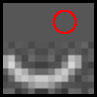
\includegraphics[scale=1.7]{img/trust_ex1}
\hspace{4em}
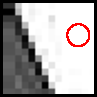
\includegraphics[scale=1.7]{img/trust_ex2}
\end{center}

\end{frame}

%%%%%%%%%%%%%%%%%%%%%%%%%%%%%%%%%%%%%%%%%%%%%%%%%%%%%%%%%%%%%%%%%%%%%%%%%%%%
\begin{frame}{Quantifying trust}
Assign a ``trust'' level to each pixel in the observed image: $T(s) \in [0, 1]$.

We do so by quantifying the consistency in pixel values around $s$.
\\[3ex]
\pause
We use:
\[ T(s) = 1 - \frac{1}{8(2\kappa-\kappa^2)} \sum_{t \sim s}M(|y_s-y_t|), \]
where
\[ M(\delta) = \begin{cases}
\delta^2 & \delta < \kappa \\
\kappa^2 + 2\kappa(\delta - \kappa) & \text{otherwise}

\end{cases} \]

\end{frame}

%%%%%%%%%%%%%%%%%%%%%%%%%%%%%%%%%%%%%%%%%%%%%%%%%%%%%%%%%%%%%%%%%%%%%%%%%%%%
\begin{frame}{How We Use Trust}
\textbf{Main Idea: If we trust a pixel, we should be less willing to update it in a way that increases the image's energy.}
\\[2ex]
\pause
Recall our acceptance probability, $e^{-\beta\Delta\!H}$.
\\[2ex]
Instead, we'll use $\left(1-T(s)\right)e^{-\beta\Delta\!H}$.
\end{frame}

%%%%%%%%%%%%%%%%%%%%%%%%%%%%%%%%%%%%%%%%%%%%%%%%%%%%%%%%%%%%%%%%%%%%%%%%%%%%%%%%%%%%%
\begin{frame}{Random Walk With Trust Results}
\centering
\begin{tabular}{c@{\hspace{.5em}}c@{\hspace{.5em}}c}
Original image & Noisy Data & MAP estimate \\[2ex]

\includegraphics[width=9.5em]{results/bw-star} 
&\includegraphics[width=9.5em]{results/bw-star-tmp}
&\includegraphics[width=9.5em]{results/bw-star-trust}
\end{tabular}
\end{frame}

%%%%%%%%%%%%%%%%%%%%%%%%%%%%%%%%%%%%%%%%%%%%%%%%%%%%%%%%%%%%%%%%%%%%%%%%%%%%
\begin{frame}{Parameters}
Our algorithm contains multiple parameters:
\[ \theta, \gamma, \alpha, \tau, \kappa \]
%The parameters interact in complicated ways; ideal parameter estimation is left as an exercise for the comps group next year.
% As we saw before, they way they affect the MAP estimate is not straightforward.
\begin{itemize}
\pause \item $h(s) = f(s) + \theta d(s)$
\pause \item $\gamma$ and $\alpha$ tune the neighbor penalty function
\pause \item $\tau$ tunes the cooling schedule
\pause \item $\kappa$ tunes the trust estimation
\end{itemize}
The MAP estimate is relatively sensitive to parameter changes.
\\[2ex]
Optimization for general inputs is a huge problem to tackle.
\end{frame}

%%%%%%%%%%%%%%%%%%%%%%%%%%%%%%%%%%%%%%%%%%%%%%%%%%%%%%%%%%%%%%%%%%%%%%%%%%%%
\begin{frame}{Back to color}
Quick and dirty approach:
\begin{itemize}
\item Split color images into a grid for R, a grid for G, and  grid for B.
\item Restore each channel independently.
\item Recombine.
\end{itemize} 
\end{frame}

%%%%%%%%%%%%%%%%%%%%%%%%%%%%%%%%%%%%%%%%%%%%%%%%%%%%%%%%%%%%%%%%%%%%%%%%%%%%
\begin{frame}{A quick recap}
\begin{block}{}
\begin{itemize}
\pause \item Build an energy function $H(x)$ to rate an arbitrary image $x$ with respect to an observed image
\pause \item Take a probabilistic approach to find the minimizer of $H$
\pause \item Construct a distribution based on $H(x) \rightarrow \Pi(x) \propto e^{-H(x)}$ 
\pause \item Sample with simulated annealing (with appropriate cooling schedule) $\rightarrow$ the mode of the distribution (and the minimizer of $H$)
\pause \item Empirical adaptations (cooling schedule modified, trust, etc.)
\end{itemize}
\end{block}
\end{frame}


%%%%%%%%%%%%%%%%%%%%%%%%%%%%%%%%%%%%%%%%%%%%%%%%%%%%%%%%%%%%%%%%%%%%%%%%%%%%
\section{Results}

%%%%%%%%%%%%%%%%%%%%%%%%%%%%%%%%%%%%%%%%%%%%%%%%%%%%%%%%%%%%%%%%%%%%%%%%%%%%
\begin{frame}{Restored star}
\centering
Noisy data
\\
\includegraphics[height=40ex]{results/star-tmp} 
\end{frame}
\begin{frame}{Restored star}
\centering
MAP estimate\vphantom{y}
\\
\includegraphics[height=40ex]{results/star-fixed} 
\end{frame}
\begin{frame}{Restored star}
\centering
Original image
\\
\includegraphics[height=40ex]{results/star} 
\end{frame}

%%%%%%%%%%%%%%%%%%%%%%%%%%%%%%%%%%%%%%%%%%%%%%%%%%%%%%%%%%%%%%%%%%%%%%%%%%%%
\begin{frame}{On a Photo?}
\centering
Noisy data
\\
\includegraphics[height=40ex]{results/lena-tmp} 
\end{frame}
\begin{frame}{On a Photo?}
\centering
MAP estimate\vphantom{y}
\\
\includegraphics[height=40ex]{results/lena-fixed}
\end{frame}
\begin{frame}{On a Photo?}
\centering
Original image
\\
\includegraphics[height=40ex]{results/lena} 
\end{frame}

%%%%%%%%%%%%%%%%%%%%%%%%%%%%%%%%%%%%%%%%%%%%%%%%%%%%%%%%%%%%%%%%%%%%%%%%%%%%
\begin{frame}{Pusheen}
\centering
Noisy data
\\
\includegraphics[height=40ex]{results/pusheen-tmp} 
\end{frame}
\begin{frame}{Pusheen}
\centering
MAP estimate\vphantom{y}
\\
\includegraphics[height=40ex]{results/pusheen-fixed}
\end{frame}
\begin{frame}{Pusheen}
\centering
Original image
\\
\includegraphics[height=40ex]{results/pusheen} 
\end{frame}

%%%%%%%%%%%%%%%%%%%%%%%%%%%%%%%%%%%%%%%%%%%%%%%%%%%%%%%%%%%%%%%%%%%%%%%%%%%%
\begin{frame}{Text}
\centering
Original image
\\
\includegraphics[height=37ex]{results/lorem} 
\end{frame}
\begin{frame}{Text}
\centering
Noisy data
\\
\includegraphics[height=37ex]{results/lorem-tmp} 
\end{frame}
\begin{frame}{Text}
\centering
MAP estimate\vphantom{y}
\\
\includegraphics[height=37ex]{results/lorem-fixed}
\end{frame}
\begin{frame}{Text}
\centering
Original image
\\
\includegraphics[height=37ex]{results/lorem} 
\end{frame}

%%%%%%%%%%%%%%%%%%%%%%%%%%%%%%%%%%%%%%%%%%%%%%%%%%%%%%%%%%%%%%%%%%%%%%%%%%%%
\begin{frame}{Illustrations}
\centering
Noisy data
\\
\includegraphics[height=40ex]{results/milk-tmp} 
\end{frame}
\begin{frame}{Illustrations}
\centering
MAP estimate\vphantom{y}
\\
\includegraphics[height=40ex]{results/milk-fixed}
\end{frame}
\begin{frame}{Illustrations}
\centering
Original image
\\
\includegraphics[height=40ex]{results/milk} 
\end{frame}

%%%%%%%%%%%%%%%%%%%%%%%%%%%%%%%%%%%%%%%%%%%%%%%%%%%%%%%%%%%%%%%%%%%%%%%%%%%%
\begin{frame}{The Last Pixelbender}
\centering
Noisy data
\\
\includegraphics[height=40ex]{results/aang2-tmp} 
\end{frame}
\begin{frame}{The Last Pixelbender}
\centering
MAP estimate\vphantom{y}
\\
\includegraphics[height=40ex]{results/aang2-fixed}
\end{frame}
\begin{frame}{The Last Pixelbender}
\centering
Original image
\\
\includegraphics[height=40ex]{results/aang2} 
\end{frame}

%%%%%%%%%%%%%%%%%%%%%%%%%%%%%%%%%%%%%%%%%%%%%%%%%%%%%%%%%%%%%%%%%%%%%%%%%%%%
\begin{frame}{The Last Pixelbender}
\centering
Noisy data
\\
\includegraphics[height=40ex]{results/aang1-tmp} 
\end{frame}
\begin{frame}{The Last Pixelbender}
\centering
MAP estimate\vphantom{y}
\\
\includegraphics[height=40ex]{results/aang1-fixed}
\end{frame}
\begin{frame}{The Last Pixelbender}
\centering
Original image
\\
\includegraphics[height=40ex]{results/aang1} 
\end{frame}

% %%%%%%%%%%%%%%%%%%%%%%%%%%%%%%%%%%%%%%%%%%%%%%%%%%%%%%%%%%%%%%%%%%%%%%%%%%%%
% \begin{frame}{How about our Bieber pic?}
% \centering
% Noisy data
% \\
% \includegraphics[height=40ex]{results/bieber} 
% \end{frame}
% \begin{frame}{How about our Bieber pic?}
% \centering
% MAP estimate\vphantom{y}
% \\
% \includegraphics[height=40ex]{results/bieber-fixed}
% \end{frame}

%%%%%%%%%%%%%%%%%%%%%%%%%%%%%%%%%%%%%%%%%%%%%%%%%%%%%%%%%%%%%%%%%%%%%%%%%%%%
\begin{frame}{How About Bob?!}
\centering
Noisy data
\\
\includegraphics[height=40ex]{results/bob-tmp} 
\end{frame}
\begin{frame}{How About Bob?!}
\centering
MAP estimate\vphantom{y}
\\
\includegraphics[height=40ex]{results/bob-fixed}
\end{frame}
\begin{frame}{How About Bob?!}
\centering
Original image
\\
\includegraphics[height=40ex]{results/bob} 
\end{frame}

%%%%%%%%%%%%%%%%%%%%%%%%%%%%%%%%%%%%%%%%%%%%%%%%%%%%%%%%%%%%%%%%%%%%%%%%%%%%
\begin{frame}{Thank You!}
\begin{center}
Bob Dobrow \& the entire Math Department
%(And the CS Department)
%(And the Department of Physics and Astronomy)
\\[2ex]
Those who attended our practice talk
\\[2ex]
Families and Friends
\\[2ex]
Markov, Gibbs, Bayes, Geman, other Geman, Hammersley, and Clifford
\\[2ex]
And \textbf{YOU}, our audience!
\end{center}
\end{frame}

%%%%%%%%%%%%%%%%%%%%%%%%%%%%%%%%%%%%%%%%%%%%%%%%%%%%%%%%%%%%%%%%%%%%%%%%%%%%
\begin{frame}{Questions?}
\vspace{-1ex}
\begin{center}
\includegraphics[scale=0.7]{img/hammersley-clifford_cats} 
\end{center}
\end{frame}

%%%%%%%%%%%%%%%%%%%%%%%%%%%%%%%%%%%%%%%%%%%%%%%%%%%%%%%%%%%%%%%%%%%%%%%%%%%%
\begin{frame}{References}
\small{
"Image Analysis, Random Fields and Markov Chain Monte Carlo Methods" by Gerhard Winkler, Springer, 2nd edition, 2003

"Stochastic Relaxation, Gibbs Distributions, and the Bayesian Restoration of Images", by Stuart Geman, Donald Geman, 1984

"Simulated Annealing" by Dimitris Bertsimas, John Tsitsiklism, 1993

"Novel Bayesian deringing method in image interpolation and compression using a SGLI prior" by Cheolkon Jung, Licheng Jiao, 2010

"Improved image decompression for reduced transform coding artifacts" by Thomas P. O'Rourke, Robert L. Stevenson, 2014

"Artifact Reduction in Low Bit Rate DCT-Based Image Compression" by Jiebo Luo, Chang Wen Chen, Kevin J. Parker, and Thomas S. Huang, 1996
}
\end{frame}

%%%%%%%%%%%%%%%%%%%%%%%%%%%%%%%%%%%%%%%%%%%%%%%%%%%%%%%%%%%%%%%%%%%%%%%%%%%%
\end{document}